\begin{frame}{Representações de Regiões}
    \begin{itemize} \setlength\itemsep{1em}
        \item Malha de quadrados
        
    \end{itemize}
    \begin{figure}[H]
        \centering
        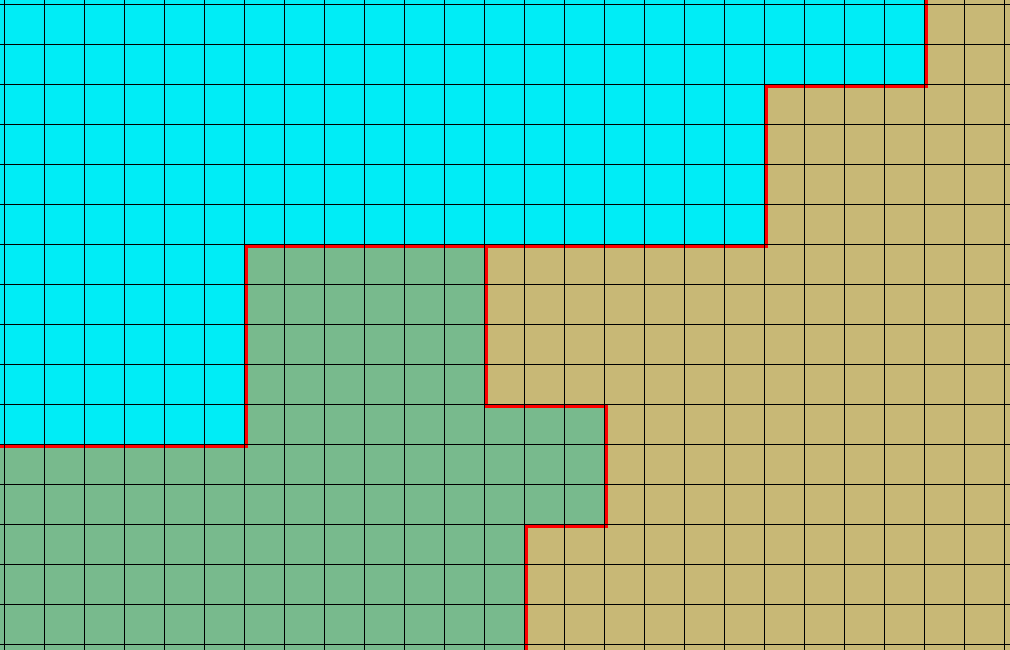
\includegraphics[width=.5\textwidth, height=.5\textheight]{img/squadStripBiomes}
        \caption{Malha de quadrados com divisão entre três Biomas.}
        \label{fig:squadStripBiomes}
    \end{figure}
\end{frame}

\begin{frame}{Representações de Regiões}
    \begin{itemize} \setlength\itemsep{1em}
        \item Malha de triângulos
        
    \end{itemize}
    \begin{figure}[H]
        \centering
        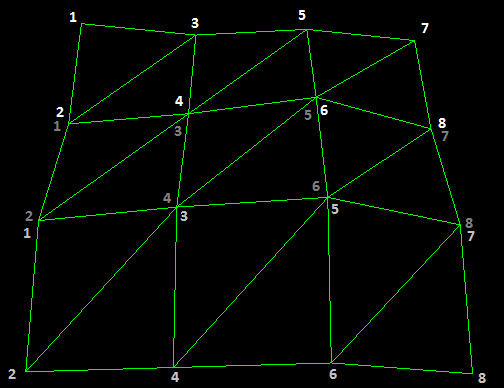
\includegraphics[width=.5\textwidth, height=.5\textheight]{img/triangle_strips}
        \caption{Malha de triângulos com altura nos vértices.}
        \label{fig:triangle_strip}
    \end{figure}
\end{frame}

\begin{frame}{Representações de Regiões}
    \begin{itemize} \setlength\itemsep{1em}
        \item Diagrama de Voronoi
        
    \end{itemize}
    \begin{figure}[H]
        \centering
        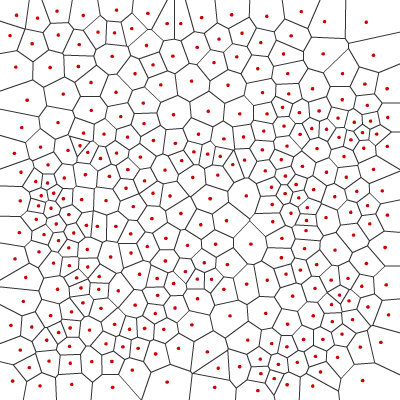
\includegraphics[width=.5\textwidth, height=.5\textheight]{img/voronoi-2-lloyd}
        \caption{Diagrama de Voronoi com Lloyd's aplicado. Por \cite{patel2010polygonal}}
        \label{fig:voronoi-2-lloyd}
    \end{figure}
\end{frame}